\documentclass[11pt]{article}

\usepackage[margin=1in]{geometry}
\usepackage[T1]{fontenc}
\usepackage{lmodern}
\usepackage{microtype}
\usepackage{amsmath,amssymb,amsthm,mathtools}
\usepackage[dvipsnames]{xcolor}
\usepackage[most]{tcolorbox}
\usepackage{tikz}
\usetikzlibrary{decorations.markings}
\usepackage{enumitem}
\usepackage{tocloft}
\usepackage[hidelinks]{hyperref}

\definecolor{courseblue}{HTML}{1F4E79}
\definecolor{lightblue}{HTML}{EAF2F8}
\definecolor{lightgreen}{HTML}{EAF7EA}
\definecolor{lightpink}{HTML}{FCE8EF}
\definecolor{lightyellow}{HTML}{FFF8D6}
\definecolor{warningyellow}{HTML}{D6A000}
\definecolor{exercisebg}{HTML}{D6E6F5}
\definecolor{exerciseframe}{HTML}{1F4E79}
\definecolor{examplebg}{HTML}{F4FAFE}
\definecolor{exampleframe}{HTML}{85C1E9}
\definecolor{darkgray}{HTML}{333333}
\definecolor{lightorange}{HTML}{FDEBD8}
\definecolor{orangeframe}{HTML}{E08A3C}

\setlength{\parindent}{0pt}
\setlength{\parskip}{0.65em}
\setlist[itemize]{topsep=0.25em,itemsep=0.15em}
\renewcommand{\cftsecleader}{\cftdotfill{\cftdotsep}}
\renewcommand{\cftsubsecleader}{\cftdotfill{\cftdotsep}}

\theoremstyle{plain}
\newtheorem{theorem}{Theorem}[section]
\newtheorem{proposition}[theorem]{Proposition}
\newtheorem{lemma}[theorem]{Lemma}
\newtheorem{corollary}[theorem]{Corollary}
\theoremstyle{definition}
\newtheorem{definition}[theorem]{Definition}
\newtheorem{example}[theorem]{Example}
\newtheorem{exercise}[theorem]{Exercise}
\theoremstyle{remark}
\newtheorem*{remark}{Remark}
\newtheorem*{fact}{Fact}
\newtheorem*{warning}{Warning}

\tcolorboxenvironment{definition}{
  enhanced,
  unbreakable,
  colback=lightgreen,
  colframe=ForestGreen,
  boxrule=0.7pt,
  arc=2pt,
  left=6pt,
  right=6pt,
  top=5pt,
  bottom=5pt
}

\tcolorboxenvironment{warning}{
  enhanced,
  colback=lightyellow,
  colframe=warningyellow,
  boxrule=0.7pt,
  arc=2pt,
  left=6pt,
  right=6pt,
  top=5pt,
  bottom=5pt
}

\tcolorboxenvironment{exercise}{
  enhanced,
  colback=exercisebg,
  colframe=exerciseframe,
  boxrule=1pt,
  arc=2pt,
  left=6pt,
  right=6pt,
  top=5pt,
  bottom=5pt
}

\tcolorboxenvironment{example}{
  enhanced,
  colback=examplebg,
  colframe=exampleframe,
  boxrule=0.7pt,
  arc=2pt,
  left=6pt,
  right=6pt,
  top=5pt,
  bottom=5pt
}

\numberwithin{equation}{section}

\newcommand{\be}{\begin{eqnarray}}
\newcommand{\ee}{\end{eqnarray}}
\newcommand{\C}{\mathbb{C}}
\newcommand{\R}{\mathbb{R}}
\newcommand{\N}{\mathbb{N}}

\DeclareMathOperator{\Hol}{\mathcal{H}\mathrm{ol}}
\DeclareMathOperator{\Real}{Re}
\DeclareMathOperator{\Imag}{Im}
\newcommand{\A}{\mathcal{A}}
\newcommand{\CT}{\C[[T]]}
\newcommand{\CLT}{\C((T))}
\tcbset{breakable}
\begin{document}

\begin{center}
  \colorbox{lightblue}{%
    \begin{minipage}{0.94\textwidth}
      \vspace{0.55em}
      \begin{tabular*}{\textwidth}{@{\extracolsep{\fill}}lr}
        {\color{courseblue}\bfseries\LARGE Lecture 12} &
        {\color{courseblue}\bfseries\LARGE MATH 411}\\[0.35em]
        \textbf{Fall 2026} & \textbf{Date: Oct 2, 2026}\\
        & \textbf{Instructor: Manish Patnaik}
      \end{tabular*}
      \vspace{0.45em}
    \end{minipage}}
\end{center}

\setcounter{tocdepth}{1}
\tableofcontents
\vspace{0.45em}

\section{Review of path integrals and estimates}
Recall the following definitions and estimates from Lecture~11. Let
$U\subseteq\C$ be open.

\begin{definition}[Piecewise continuously differentiable path]
A curve $\gamma\colon[a,b]\to U$ is \emph{piecewise continuously differentiable}
if it is continuous on $[a,b]$ and there is a finite partition
$a=t_0<t_1<\cdots<t_m=b$ such that $\gamma$ is continuously differentiable
on each $[t_{j-1},t_j]$, with one-sided derivatives at the endpoints.
Unless said otherwise, a \emph{path} means such a curve. Its derivative
need not exist at the joining points $t_1,\ldots,t_{m-1}$.
\end{definition}

\begin{definition}[Path integral]
\label{def:path-int}
For $f$ continuous on $U$ and $\gamma\colon[a,b]\to U$ a path, write
$\gamma(t)=u(t)+iv(t)$, so $\gamma'(t)=u'(t)+iv'(t)$ on each $C^1$ piece. Then
\be
 \int_\gamma f=\int_\gamma f\,dz:=\int_a^bf\bigl(\gamma(t)\bigr)\,\gamma'(t)\,dt.
\ee
\end{definition}

\begin{proposition}[Triangle inequality]
\label{prop:basic-est}
For continuous $F\colon[a,b]\to\C$,
\be
 \left|\int_a^bF(t)\,dt\right|\leq\int_a^b|F(t)|\,dt.
\ee
\end{proposition}

\begin{proposition}[ML estimate]
\label{prop:ML}
For a path $\gamma\colon[a,b]\to\C$, let
\be
 L(\gamma)=\text{arclength of }\gamma=\int_a^b|\gamma'(t)|\,dt.
\ee
Then
\be
 \left|\int_\gamma f\right|\leq\Bigl(\sup_{z\in\gamma([a,b])}|f(z)|\Bigr)\cdot L(\gamma).
\ee
\end{proposition}

\begin{proof}
Why? Since $\int_\gamma f=\int_a^bf\bigl(\gamma(t)\bigr)\,\gamma'(t)\,dt$, the
basic estimate above gives
\be
 \left|\int_\gamma f\right|\leq\int_a^b\bigl|f\bigl(\gamma(t)\bigr)\bigr|\,|\gamma'(t)|\,dt
 \leq\sup_{z\in\gamma([a,b])}|f(z)|\int_a^b|\gamma'(t)|\,dt.
\ee
\end{proof}

\section{The Cauchy--Goursat theorem}
Let $U\subseteq\C$ be open and $f$ holomorphic on $U$. Let $R$ be any
(closed) rectangle in $U$ with sides parallel to the axes, and write
$\partial R$ for its boundary, traversed counterclockwise.

\begin{center}
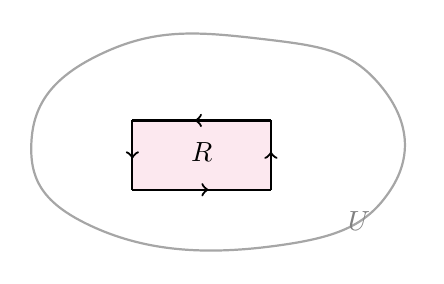
\begin{tikzpicture}[scale=0.8,decoration={markings,mark=at position 0.55 with {\arrow{>}}}]
  \draw[thick,gray!70] plot[smooth cycle,tension=0.8]
    coordinates {(-2.8,0.2) (-1.6,1.6) (0.8,1.8) (2.7,1.1) (2.9,-0.6) (1.0,-1.5) (-1.8,-1.2)};
  \fill[lightpink] (-1.2,-0.6) rectangle (1.0,0.5);
  \draw[thick,postaction={decorate}] (-1.2,-0.6) -- (1.0,-0.6);
  \draw[thick,postaction={decorate}] (1.0,-0.6) -- (1.0,0.5);
  \draw[thick,postaction={decorate}] (1.0,0.5) -- (-1.2,0.5);
  \draw[thick,postaction={decorate}] (-1.2,0.5) -- (-1.2,-0.6);
  \node at (-0.1,0) {$R$};
  \node[gray] at (2.4,-1.1) {$U$};
\end{tikzpicture}
\end{center}

\begin{theorem}[Cauchy--Goursat]
\label{thm:goursat}
$\displaystyle\int_{\partial R}f=0.$
\end{theorem}

% Handwritten page 4.
\begin{proof}
There are three steps. We don't use that $f$ is holomorphic in Step~1.

\textbf{Step 1: subdivide.} Cut $R$ into four congruent subrectangles
$R_1,R_2,R_3,R_4$ by bisecting its sides, and orient each boundary
counterclockwise.

\begin{center}
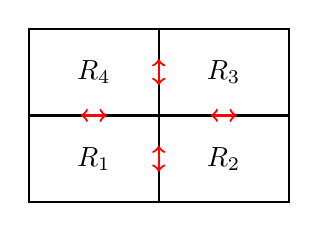
\begin{tikzpicture}[scale=1.1,decoration={markings,mark=at position 0.55 with {\arrow{>}}}]
  \draw[thick] (0,0) rectangle (3,2);
  \draw[thick] (1.5,0) -- (1.5,2);
  \draw[thick] (0,1) -- (3,1);
  \node at (0.75,0.5) {$R_1$}; \node at (2.25,0.5) {$R_2$};
  \node at (2.25,1.5) {$R_3$}; \node at (0.75,1.5) {$R_4$};
  \draw[red,thick,<->] (1.5,0.35) -- (1.5,0.65);
  \draw[red,thick,<->] (1.5,1.35) -- (1.5,1.65);
  \draw[red,thick,<->] (0.6,1) -- (0.9,1);
  \draw[red,thick,<->] (2.1,1) -- (2.4,1);
\end{tikzpicture}
\end{center}

Each interior edge is traversed twice, in opposite directions, so those
contributions cancel and
\be
 \int_{\partial R}f=\int_{\partial R_1}f+\int_{\partial R_2}f+\int_{\partial R_3}f+\int_{\partial R_4}f.
\ee
Hence
\be
 \left|\int_{\partial R}f\right|\leq\sum_{i=1}^{4}\left|\int_{\partial R_i}f\right|,
\ee
so there exists some subrectangle $R^{(1)}\in\{R_1,\dots,R_4\}$ such that
\be
 \left|\int_{\partial R^{(1)}}f\right|\geq\frac14\left|\int_{\partial R}f\right|.
\ee

% Handwritten page 5.
Apply the same reasoning to $\int_{\partial R^{(1)}}f$, i.e.\ break up
$R^{(1)}$ into four subrectangles, and argue that there is one of them,
$R^{(2)}$, with
\be
 \left|\int_{\partial R^{(2)}}f\right|\geq\frac14\left|\int_{\partial R^{(1)}}f\right|
 \ \Longrightarrow\
 \left|\int_{\partial R^{(2)}}f\right|\geq\frac14\cdot\frac14\left|\int_{\partial R}f\right|.
\ee

\begin{center}
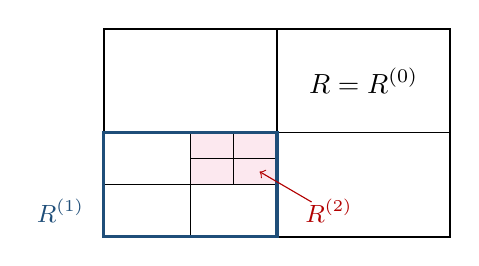
\begin{tikzpicture}[scale=1.1]
  \draw[thick] (0,0) rectangle (4,2.4);
  \draw (2,0) -- (2,2.4); \draw (0,1.2) -- (4,1.2);
  \draw (1,0) -- (1,1.2); \draw (0,0.6) -- (2,0.6);
  \fill[lightpink] (1,0.6) rectangle (2,1.2);
  \draw (1,0.6) rectangle (2,1.2);
  \draw (1.5,0.6) -- (1.5,1.2); \draw (1,0.9) -- (2,0.9);
  \draw[very thick,courseblue] (0,0) rectangle (2,1.2);
  \node[courseblue,font=\small] at (-0.5,0.3) {$R^{(1)}$};
  \node[red!70!black,font=\small] at (2.6,0.3) {$R^{(2)}$};
  \draw[->,red!70!black] (2.4,0.4) -- (1.8,0.75);
  \node at (3,1.8) {$R=R^{(0)}$};
\end{tikzpicture}
\end{center}

Continue to find rectangles $R=R^{(0)}\supset R^{(1)}\supset R^{(2)}\supset\cdots$ such that
\begin{tcolorbox}[enhanced,colback=lightgreen,colframe=ForestGreen,boxrule=0.7pt,arc=2pt]
\be
 \left|\int_{\partial R^{(n)}}f\right|\geq\frac1{4^n}\left|\int_{\partial R}f\right|.
 \label{eq:4n}
\ee
\end{tcolorbox}

\textbf{Step 2: the rectangles shrink to a point.} Let
\be
 L_n=\text{arclength of }\partial R^{(n)}\ (\text{the perimeter of this rectangle}),\qquad
 d_n=\operatorname{diam}\bigl(R^{(n)}\bigr),
\ee
where the diameter is the maximum distance between two points of
$R^{(n)}$. Since each step halves the side lengths, we find
\be
 L_n=\frac1{2^n}L_0,\qquad d_n=\frac1{2^n}d_0.
\ee

% Handwritten page 6.
\emph{Claim.} $\bigcap_{n=1}^{\infty}R^{(n)}$ consists of a single point.

Since $d_n\to0$, there cannot be two distinct points in
$\bigcap_nR^{(n)}$. But why is there one point? Pick $\alpha_j\in R^{(j)}$.
For $j,k\geq n$ both $\alpha_j,\alpha_k$ lie in $R^{(n)}$, so
$|\alpha_j-\alpha_k|\leq d_n\to0$: the sequence $\{\alpha_j\}$ is Cauchy.
Therefore it has a limit $z_0$. For each $n$, the tail $\{\alpha_j\}_{j\geq n}$
lies in $R^{(n)}$, which is closed (it contains the limit of any Cauchy
sequence it contains), so $z_0\in R^{(n)}$. Thus
$z_0\in\bigcap_{n}R^{(n)}$.

\textbf{Step 3: use holomorphicity.} Now we want to input that $f$ is
holomorphic. We pick $z_0$ to be the point $\bigcap_{n=1}^{\infty}R^{(n)}$.
Then $f$ being holomorphic at $z_0\in U$ means: there is a function
$\varphi(z)$ defined on a neighbourhood $V\ni z_0$, with
$\lim_{z\to z_0}\varphi(z)=0$, $\varphi(z_0)=0$, and such that
\begin{tcolorbox}[enhanced,colback=lightgreen,colframe=ForestGreen,boxrule=0.7pt,arc=2pt]
\[ f(z)=f(z_0)+f'(z_0)(z-z_0)+\varphi(z)(z-z_0)\qquad(z\in V). \]
\end{tcolorbox}
Note that the function $\varphi$ is continuous on $V$: this is certainly true at $z=z_0$, and for $z\neq z_0$ it equals $\frac{f(z)-f(z_0)}{z-z_0}-f'(z_0).$ But $f$ is
continuous, being $\C$-differentiable.

% Handwritten page 7.
\noindent
\begin{minipage}[c]{0.62\textwidth}
Since $d_n\to0$ and $z_0\in R^{(n)}$, we may choose $n$ large so that
$R^{(n)}\subseteq V$. Then
\begin{align*}
 \int_{\partial R^{(n)}}f
 &=\underbrace{\int_{\partial R^{(n)}}f(z_0)\,dz}_{0}
 +\underbrace{\int_{\partial R^{(n)}}f'(z_0)(z-z_0)\,dz}_{0}\\
 &\qquad+\int_{\partial R^{(n)}}\varphi(z)(z-z_0)\,dz,
\end{align*}
where the first two integrals vanish because integrals of polynomials
over closed paths vanish (Lecture~11).
\end{minipage}\hfill
\begin{minipage}[c]{0.34\textwidth}
\centering
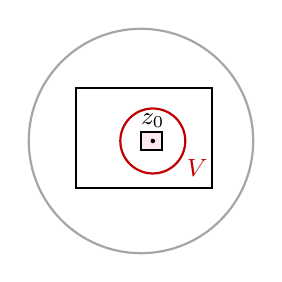
\begin{tikzpicture}[scale=0.75]
  \draw[thick,gray!70] (0,0) circle (1.9);
  \draw[thick] (-1.1,-0.8) rectangle (1.2,0.9);
  \draw[red!75!black,thick] (0.2,0.0) circle (0.55);
  \node[red!75!black,font=\small] at (0.95,-0.45) {$V$};
  \draw[thick,fill=lightpink] (0.0,-0.15) rectangle (0.35,0.15);
  \fill (0.2,0.0) circle (1.1pt);
  \node[font=\small] at (0.2,0.35) {$z_0$};
\end{tikzpicture}
\end{minipage}

So
\be
 \int_{\partial R^{(n)}}f=\int_{\partial R^{(n)}}\varphi(z)(z-z_0)\,dz
 \qquad\text{for any $n$ sufficiently large.}
\ee
Combining with \eqref{eq:4n} and the ML-estimate,
\begin{align*}
 \left|\int_{\partial R}f\right|
 &\leq4^n\left|\int_{\partial R^{(n)}}f\right|
 \leq4^n\left|\int_{\partial R^{(n)}}\varphi(z)(z-z_0)\,dz\right|\\
 &\leq4^n\cdot\sup_{z\in\partial R^{(n)}}\bigl|\varphi(z)\bigr|\,|z-z_0|\cdot L_n
 \qquad(L_n=\text{arclength of }\partial R^{(n)})\\
 &\leq4^n\cdot\sup_{z\in\partial R^{(n)}}|\varphi(z)|\cdot\sup_{z\in\partial R^{(n)}}|z-z_0|\cdot\frac1{2^n}L_0\\
 &\leq4^n\cdot\operatorname{diam}\bigl(R^{(n)}\bigr)\cdot\sup_{z\in\partial R^{(n)}}|\varphi(z)|\cdot\frac1{2^n}L_0
 \qquad(z_0\in R^{(n)})\\
% Handwritten page 8.
 &\leq4^n\cdot\frac1{2^n}d_0\cdot\sup_{z\in\partial R^{(n)}}|\varphi(z)|\cdot\frac1{2^n}L_0
 =C\cdot\sup_{z\in\partial R^{(n)}}|\varphi(z)|,
\end{align*}
with $C=d_0L_0$ independent of $n$. As $n\to\infty$, every point of
$\partial R^{(n)}$ is within $d_n\to0$ of $z_0$, and $\varphi(z)\to0$ as
$|z-z_0|\to0$. So the right-hand side tends to $0$, and hence
$\int_{\partial R}f=0$.
\end{proof}

\begin{remark}
The factor $4^n$ lost in Step~1 is exactly compensated by the factors
$\frac1{2^n}$ from the diameter and the perimeter in Step~3. The theorem
really uses only that $f$ is $\C$-differentiable at each point; we did not
assume $f'$ is continuous.
\end{remark}

\begin{exercise}
	
	
\end{exercise}
%
%\section{Primitives}
%\begin{definition}[Primitive]
%Let $f$ be a continuous function on an open set $U\subseteq\C$. A
%\emph{primitive} for $f$ (or \emph{holomorphic primitive}) is a function
%$g\colon U\to\C$ such that $g$ is holomorphic and
%\be
% g'=f\qquad\text{on }U.
%\ee
%\end{definition}
%
%\begin{example}[Analytic functions have local primitives]
%\label{ex:local-prim}
%Recall: if $f$ is analytic on $U$, so
%\be
% f(z)=\sum a_n(z-z_0)^n\qquad\text{for $z$ near $z_0$},
%\ee
%then $f'(z)$ exists and is computed term by term. But we can also
%``integrate term by term'' to get the series
%\be
% g(z)=\sum_n\frac{a_n}{n+1}(z-z_0)^{n+1}.
%\ee
%What do we know about this series? Its coefficient of $(z-z_0)^{n+1}$ is
%$\frac{a_n}{n+1}$, and
%\be
% \limsup_n\left|\frac{a_n}{n+1}\right|^{1/n}
% =\limsup_n\frac{|a_n|^{1/n}}{(n+1)^{1/n}}
% =\limsup_n|a_n|^{1/n},
%\ee
%since $(n+1)^{1/n}\to1$. (Shifting the index by one does not change the
%radius of convergence.) Therefore $g(z)$ is also convergent for $z$ near
%$z_0$, so
%\be
% g(z)\ \text{analytic}\ \Longrightarrow\ \text{holomorphic, and}\ g'=f
%\ee
%by term-by-term differentiation. So $g$ is a primitive for $f$ on a disc
%around $z_0$.
%\end{example}

\end{document}
